\section{Background}

X-rays are a type of ionizing electromagnetic radiation with typical energies in the \unit{\kilo\electronvolt} range. Their
production inside an X-ray tube relies on the electrostatic acceleration of electrons which then interact with the anode material. The main
mechanisms for the emission of energetic photons are the continuous bremsstrahlung resulting from electron deceleration as well as a
discrete component emitted after penetration of the inner atomic shells \cite{McMorrow_2011_1, McMorrow_2011_2}.



\subsection{Refractive index}

In classical ray optics, the laws of reflection and refraction are
\begin{align}
	\theta_i = \theta_r \: , && n_1 \cos\theta_i = n_2 \cos\theta_t \: ,
	\label{eqn:snell}
\end{align}
where $n_1$ and $n_2$ are the refractive indices of the two media and $\theta_i, \theta_r, \theta_t$ are the angles of incidence, reflection
and transmission as shown in Figure \ref{fig:fresnel}.

\begin{figure}[H]
	\centering
	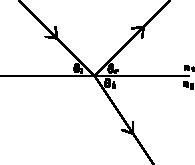
\includegraphics[width=0.33\textwidth]{content/graphics/fresnel.pdf}
	\caption{Depiction of reflection and refraction of light rays on a smooth surface.}
	\label{fig:fresnel}
\end{figure}

For X-rays, the refractive index can usually be written as
\begin{equation*}
	n_2 \equiv n = 1 - \delta \pm i\beta \: ,
\end{equation*}
with the extinction coefficient $\beta > 0$ measuring the exponential absorption and a small correction $\delta > 0$ to the real part.
The choice of $\pm$ depends on the sign convention for the wave vector. From $1 - \delta < 1$ further follows that the phase velocity
of X-rays can exceed the speed of light in vacuum $c$. Because information travels at the group velocity, this does not violate special
relativity. Assuming air or vacuum as the surrounding medium, one can set
\begin{equation*}
	n_1 \equiv 1 \: ,
\end{equation*}
resulting in a transition from an optically thick to a thin medium. Accordingly, total reflection occurs for small angles
$\theta_i < \theta_c,$ with
\begin{equation*}
	\theta_c = \arccos n
\end{equation*}
defining the critical angle. Proceeding in the small angle approximation, one can expand
\begin{equation*}
	\cos\theta \cong 1 - \pfrac{1}{2} \theta^2
\end{equation*}
to second order. Rewriting Snell's law \eqref{eqn:snell} as
\begin{equation*}
	1 - \pfrac{1}{2} \theta_i^2 \cong n \left( 1 - \pfrac{1}{2}\theta_t^2 \right) = (1 - \delta \pm i\beta) \left( 1 - \pfrac{1}{2}\theta_t^2 \right)
	\cong 1 - \delta \pm i\beta - \pfrac{1}{2}\theta_t^2
\end{equation*}
yields \cite{McMorrow_2011_3} the relationship
\begin{equation}
	\theta_i \cong \sqrt{\theta_t^2 + 2\delta \mp 2i\beta} \: ,
	\label{eqn:angles}
\end{equation}
where products of $\delta, \beta, \theta_t \ll 1$ are ignored in the last step. Similarly, one identifies
\begin{equation*}
	\theta_c \cong \sqrt{2\delta \mp 2i\beta}
\end{equation*}
by setting $\theta_t = 0$ in \eqref{eqn:angles}.



\subsection{Kiessig fringes}

\cite{Kiessig_1931}

\begin{figure}[H]
	\centering
	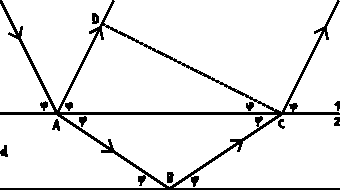
\includegraphics[width=0.55\textwidth]{content/graphics/kiessig.pdf}
	\caption{Schematic light paths inside a thin layer atop a substrate producing Kiessig oscillations according to \cite{Kiessig_1931}.}
	\label{fig:kiessig}
\end{figure}



\subsection{Fresnel coefficients}

Fresnel's formulae\footnote{In the general form given in \cite{Parratt_1954}.}



\subsection{Stratified media}

\cite{Parratt_1954}

\begin{figure}[H]
	\centering
	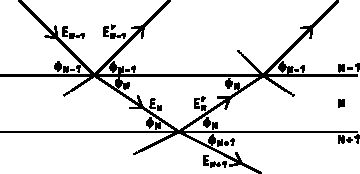
\includegraphics[width=0.66\textwidth]{content/graphics/parratt.pdf}
	\caption{Conceptual visualization of the Parratt algorithm presented in \cite{Parratt_1954}.}
	\label{fig:parratt}
\end{figure}

\cite{xray}
